\documentclass[]{article}
\usepackage{lmodern}
\usepackage{amssymb,amsmath}
\usepackage{ifxetex,ifluatex}
\usepackage{fixltx2e} % provides \textsubscript
\ifnum 0\ifxetex 1\fi\ifluatex 1\fi=0 % if pdftex
  \usepackage[T1]{fontenc}
  \usepackage[utf8]{inputenc}
\else % if luatex or xelatex
  \ifxetex
    \usepackage{mathspec}
  \else
    \usepackage{fontspec}
  \fi
  \defaultfontfeatures{Ligatures=TeX,Scale=MatchLowercase}
\fi
% use upquote if available, for straight quotes in verbatim environments
\IfFileExists{upquote.sty}{\usepackage{upquote}}{}
% use microtype if available
\IfFileExists{microtype.sty}{%
\usepackage{microtype}
\UseMicrotypeSet[protrusion]{basicmath} % disable protrusion for tt fonts
}{}
\usepackage[margin=1in]{geometry}
\usepackage{hyperref}
\hypersetup{unicode=true,
            pdftitle={Impact of biostimulants on soil nitrogen dynamics},
            pdfauthor={Mark Farrell},
            pdfborder={0 0 0},
            breaklinks=true}
\urlstyle{same}  % don't use monospace font for urls
\usepackage{color}
\usepackage{fancyvrb}
\newcommand{\VerbBar}{|}
\newcommand{\VERB}{\Verb[commandchars=\\\{\}]}
\DefineVerbatimEnvironment{Highlighting}{Verbatim}{commandchars=\\\{\}}
% Add ',fontsize=\small' for more characters per line
\usepackage{framed}
\definecolor{shadecolor}{RGB}{248,248,248}
\newenvironment{Shaded}{\begin{snugshade}}{\end{snugshade}}
\newcommand{\KeywordTok}[1]{\textcolor[rgb]{0.13,0.29,0.53}{\textbf{#1}}}
\newcommand{\DataTypeTok}[1]{\textcolor[rgb]{0.13,0.29,0.53}{#1}}
\newcommand{\DecValTok}[1]{\textcolor[rgb]{0.00,0.00,0.81}{#1}}
\newcommand{\BaseNTok}[1]{\textcolor[rgb]{0.00,0.00,0.81}{#1}}
\newcommand{\FloatTok}[1]{\textcolor[rgb]{0.00,0.00,0.81}{#1}}
\newcommand{\ConstantTok}[1]{\textcolor[rgb]{0.00,0.00,0.00}{#1}}
\newcommand{\CharTok}[1]{\textcolor[rgb]{0.31,0.60,0.02}{#1}}
\newcommand{\SpecialCharTok}[1]{\textcolor[rgb]{0.00,0.00,0.00}{#1}}
\newcommand{\StringTok}[1]{\textcolor[rgb]{0.31,0.60,0.02}{#1}}
\newcommand{\VerbatimStringTok}[1]{\textcolor[rgb]{0.31,0.60,0.02}{#1}}
\newcommand{\SpecialStringTok}[1]{\textcolor[rgb]{0.31,0.60,0.02}{#1}}
\newcommand{\ImportTok}[1]{#1}
\newcommand{\CommentTok}[1]{\textcolor[rgb]{0.56,0.35,0.01}{\textit{#1}}}
\newcommand{\DocumentationTok}[1]{\textcolor[rgb]{0.56,0.35,0.01}{\textbf{\textit{#1}}}}
\newcommand{\AnnotationTok}[1]{\textcolor[rgb]{0.56,0.35,0.01}{\textbf{\textit{#1}}}}
\newcommand{\CommentVarTok}[1]{\textcolor[rgb]{0.56,0.35,0.01}{\textbf{\textit{#1}}}}
\newcommand{\OtherTok}[1]{\textcolor[rgb]{0.56,0.35,0.01}{#1}}
\newcommand{\FunctionTok}[1]{\textcolor[rgb]{0.00,0.00,0.00}{#1}}
\newcommand{\VariableTok}[1]{\textcolor[rgb]{0.00,0.00,0.00}{#1}}
\newcommand{\ControlFlowTok}[1]{\textcolor[rgb]{0.13,0.29,0.53}{\textbf{#1}}}
\newcommand{\OperatorTok}[1]{\textcolor[rgb]{0.81,0.36,0.00}{\textbf{#1}}}
\newcommand{\BuiltInTok}[1]{#1}
\newcommand{\ExtensionTok}[1]{#1}
\newcommand{\PreprocessorTok}[1]{\textcolor[rgb]{0.56,0.35,0.01}{\textit{#1}}}
\newcommand{\AttributeTok}[1]{\textcolor[rgb]{0.77,0.63,0.00}{#1}}
\newcommand{\RegionMarkerTok}[1]{#1}
\newcommand{\InformationTok}[1]{\textcolor[rgb]{0.56,0.35,0.01}{\textbf{\textit{#1}}}}
\newcommand{\WarningTok}[1]{\textcolor[rgb]{0.56,0.35,0.01}{\textbf{\textit{#1}}}}
\newcommand{\AlertTok}[1]{\textcolor[rgb]{0.94,0.16,0.16}{#1}}
\newcommand{\ErrorTok}[1]{\textcolor[rgb]{0.64,0.00,0.00}{\textbf{#1}}}
\newcommand{\NormalTok}[1]{#1}
\usepackage{graphicx,grffile}
\makeatletter
\def\maxwidth{\ifdim\Gin@nat@width>\linewidth\linewidth\else\Gin@nat@width\fi}
\def\maxheight{\ifdim\Gin@nat@height>\textheight\textheight\else\Gin@nat@height\fi}
\makeatother
% Scale images if necessary, so that they will not overflow the page
% margins by default, and it is still possible to overwrite the defaults
% using explicit options in \includegraphics[width, height, ...]{}
\setkeys{Gin}{width=\maxwidth,height=\maxheight,keepaspectratio}
\IfFileExists{parskip.sty}{%
\usepackage{parskip}
}{% else
\setlength{\parindent}{0pt}
\setlength{\parskip}{6pt plus 2pt minus 1pt}
}
\setlength{\emergencystretch}{3em}  % prevent overfull lines
\providecommand{\tightlist}{%
  \setlength{\itemsep}{0pt}\setlength{\parskip}{0pt}}
\setcounter{secnumdepth}{0}
% Redefines (sub)paragraphs to behave more like sections
\ifx\paragraph\undefined\else
\let\oldparagraph\paragraph
\renewcommand{\paragraph}[1]{\oldparagraph{#1}\mbox{}}
\fi
\ifx\subparagraph\undefined\else
\let\oldsubparagraph\subparagraph
\renewcommand{\subparagraph}[1]{\oldsubparagraph{#1}\mbox{}}
\fi

%%% Use protect on footnotes to avoid problems with footnotes in titles
\let\rmarkdownfootnote\footnote%
\def\footnote{\protect\rmarkdownfootnote}

%%% Change title format to be more compact
\usepackage{titling}

% Create subtitle command for use in maketitle
\newcommand{\subtitle}[1]{
  \posttitle{
    \begin{center}\large#1\end{center}
    }
}

\setlength{\droptitle}{-2em}

  \title{Impact of biostimulants on soil nitrogen dynamics}
    \pretitle{\vspace{\droptitle}\centering\huge}
  \posttitle{\par}
    \author{Mark Farrell}
    \preauthor{\centering\large\emph}
  \postauthor{\par}
      \predate{\centering\large\emph}
  \postdate{\par}
    \date{12/10/2018}


\begin{document}
\maketitle

\section{Overview}\label{overview}

These data are from a pot experiment that was conducted to investigate
whether biostimulants impact on soil nitrogen (N) cycling and wheat
uptake of legume-derived N. Here, we are looking at soluble N and carbon
(C) pools over the growth period. These are presented in mg
L\textsuperscript{-1} as they are derived from soil solution samples
that were collected non-destructively using
\href{https://www.rhizosphere.com/}{Rhizon samplers}.
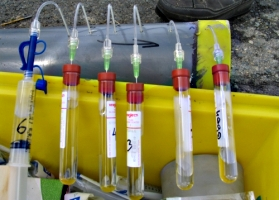
\includegraphics{https://www.rhizosphere.com/assets/images/RhizonCSSinacoreRRP.jpg}

\subsection{Initial data processing, tidying,
etc}\label{initial-data-processing-tidying-etc}

First, we need to lead tidyverse, and bring the data into the R
environment

\begin{Shaded}
\begin{Highlighting}[]
\KeywordTok{library}\NormalTok{(tidyverse)}
\KeywordTok{library}\NormalTok{(lmerTest)}
\KeywordTok{library}\NormalTok{(emmeans)}
\KeywordTok{setwd}\NormalTok{(}\StringTok{"~/DATASCHOOL/r-learning/15N-continuation/"}\NormalTok{)}
\NormalTok{raw_data <-}\StringTok{ }\KeywordTok{read_csv}\NormalTok{(}\StringTok{"data/working/15n_soil_sol.csv"}\NormalTok{)}
\end{Highlighting}
\end{Shaded}

We can now see that the data has been successfully loaded into the
environment:

\begin{Shaded}
\begin{Highlighting}[]
\NormalTok{raw_data}
\end{Highlighting}
\end{Shaded}

\begin{verbatim}
## # A tibble: 576 x 10
##    sample    trt   block   pot  days   no3   nh4    faa   tdn   doc
##    <chr>     <chr> <int> <int> <int> <dbl> <dbl>  <dbl> <dbl> <dbl>
##  1 15NSS_001 A         1    11     0  1.67  2.77  3.22   64.0  312.
##  2 15NSS_002 A         2    24     0 NA    NA    NA      61.8  298.
##  3 15NSS_003 A         3    30     0  1.64  3.92  1.34   63.5  302.
##  4 15NSS_004 A         4    42     0  1.69  4.15  0.997  62.4  285.
##  5 15NSS_005 A         5    53     0  1.69  3.7   1.58   66.8  290.
##  6 15NSS_006 A         6    68     0  1.66  4.77  1.49   56.2  238.
##  7 15NSS_007 B         1     9     0  1.64  3.59  1.43   65.7  234.
##  8 15NSS_008 B         2    13     0  1.62  4.6   1.97   57.9   NA 
##  9 15NSS_009 B         3    28     0  1.65  3.72  1.44   63.5  244.
## 10 15NSS_010 B         4    38     0  1.68  5.47  0.935  63.5  232.
## # ... with 566 more rows
\end{verbatim}

There are now several steps that need to be taken before we can start
graphing the data. Some variables need to be calculated:

\begin{itemize}
\tightlist
\item
  DIN
\item
  DON
\item
  DOC\_DON ratio
\item
  DON\_DIN ratio
\end{itemize}

Making a new variable is easy. As I forgot to give it a name, I also
re-named is using the \texttt{name} function in base R

\begin{Shaded}
\begin{Highlighting}[]
\NormalTok{with_din <-}\StringTok{ }\KeywordTok{mutate}\NormalTok{(raw_data, nh4 }\OperatorTok{+}\StringTok{ }\NormalTok{no3)}
\KeywordTok{names}\NormalTok{(with_din)[}\DecValTok{11}\NormalTok{] <-}\StringTok{ "din"}
\end{Highlighting}
\end{Shaded}

As part of this there is some cleaning that also needs to happen. In
calculating DON, we can use \texttt{case\_when()} in the mutate function
to identify values \textless{} 0 and make them 0:

\begin{Shaded}
\begin{Highlighting}[]
\NormalTok{with_don <-}\StringTok{ }\NormalTok{with_din }\OperatorTok\StringTok{ }
\StringTok{  }\KeywordTok{mutate}\NormalTok{(}\DataTypeTok{don =}\NormalTok{ tdn }\OperatorTok{-}\StringTok{ }\NormalTok{din,}
         \DataTypeTok{don_nz =} \KeywordTok{case_when}\NormalTok{(}
\NormalTok{           don }\OperatorTok{>=}\StringTok{ }\DecValTok{0} \OperatorTok{~}\StringTok{ }\NormalTok{don,}
           \OtherTok{TRUE} \OperatorTok{~}\StringTok{ }\DecValTok{0}
\NormalTok{         ))}
\end{Highlighting}
\end{Shaded}

Doing some more simple mutations calculates the ratios, but also
generates \texttt{Inf} where a divide by zero has happened

\begin{Shaded}
\begin{Highlighting}[]
\NormalTok{ratios <-}\StringTok{ }\KeywordTok{mutate}\NormalTok{(don_fixed, }\DataTypeTok{doc_don =}\NormalTok{ doc }\OperatorTok{/}\StringTok{ }\NormalTok{don )}
\NormalTok{ratios <-}\StringTok{ }\KeywordTok{mutate}\NormalTok{(ratios, }\DataTypeTok{don_din =}\NormalTok{ don }\OperatorTok{/}\StringTok{ }\NormalTok{din )}
\end{Highlighting}
\end{Shaded}

\begin{verbatim}
## # A tibble: 576 x 14
##    sample trt   block   pot  days   no3   nh4    faa   tdn   doc   din
##    <chr>  <chr> <int> <int> <int> <dbl> <dbl>  <dbl> <dbl> <dbl> <dbl>
##  1 15NSS~ A         1    11     0  1.67  2.77  3.22   64.0  312.  4.44
##  2 15NSS~ A         2    24     0 NA    NA    NA      61.8  298. NA   
##  3 15NSS~ A         3    30     0  1.64  3.92  1.34   63.5  302.  5.56
##  4 15NSS~ A         4    42     0  1.69  4.15  0.997  62.4  285.  5.84
##  5 15NSS~ A         5    53     0  1.69  3.7   1.58   66.8  290.  5.39
##  6 15NSS~ A         6    68     0  1.66  4.77  1.49   56.2  238.  6.43
##  7 15NSS~ B         1     9     0  1.64  3.59  1.43   65.7  234.  5.23
##  8 15NSS~ B         2    13     0  1.62  4.6   1.97   57.9   NA   6.22
##  9 15NSS~ B         3    28     0  1.65  3.72  1.44   63.5  244.  5.37
## 10 15NSS~ B         4    38     0  1.68  5.47  0.935  63.5  232.  7.15
## # ... with 566 more rows, and 3 more variables: don <dbl>, doc_don <dbl>,
## #   don_din <dbl>
\end{verbatim}

The \texttt{case\_when} operation above won't work here straight away to
turn \texttt{Inf} to \texttt{\textquotesingle{}NA\textquotesingle{}}

So, Alex provided a solution using to change all infinate values to NA:
\texttt{don\_fixed\$doc\_don{[}which(is.infinite(don\_fixed\$doc\_don)){]}\ \textless{}-\ NA}
I also found one on
\href{https://stackoverflow.com/questions/12188509/cleaning-inf-values-from-an-r-dataframe}{Stack
Overflow}

\begin{Shaded}
\begin{Highlighting}[]
\KeywordTok{is.na}\NormalTok{(ratios) <-}\StringTok{ }\KeywordTok{do.call}\NormalTok{(cbind,}\KeywordTok{lapply}\NormalTok{(ratios, is.infinite))}
\end{Highlighting}
\end{Shaded}

This searches the data frame, finds infinate values and replaces them
with NA

\begin{verbatim}
## # A tibble: 576 x 14
##    sample trt   block   pot  days   no3   nh4    faa   tdn   doc   din
##    <chr>  <chr> <int> <int> <int> <dbl> <dbl>  <dbl> <dbl> <dbl> <dbl>
##  1 15NSS~ A         1    11     0  1.67  2.77  3.22   64.0  312.  4.44
##  2 15NSS~ A         2    24     0 NA    NA    NA      61.8  298. NA   
##  3 15NSS~ A         3    30     0  1.64  3.92  1.34   63.5  302.  5.56
##  4 15NSS~ A         4    42     0  1.69  4.15  0.997  62.4  285.  5.84
##  5 15NSS~ A         5    53     0  1.69  3.7   1.58   66.8  290.  5.39
##  6 15NSS~ A         6    68     0  1.66  4.77  1.49   56.2  238.  6.43
##  7 15NSS~ B         1     9     0  1.64  3.59  1.43   65.7  234.  5.23
##  8 15NSS~ B         2    13     0  1.62  4.6   1.97   57.9   NA   6.22
##  9 15NSS~ B         3    28     0  1.65  3.72  1.44   63.5  244.  5.37
## 10 15NSS~ B         4    38     0  1.68  5.47  0.935  63.5  232.  7.15
## # ... with 566 more rows, and 3 more variables: don <dbl>, doc_don <dbl>,
## #   don_din <dbl>
\end{verbatim}

Finally, the finished dataframe is written to a new *.csv

\texttt{write\_csv(ratios,\ "data/processed/ratios.csv")}


\end{document}
